\documentclass[aspectratio=169]{beamer}
\usetheme{Madrid}
\usecolortheme{default}
\usepackage{booktabs,graphicx,xcolor,multirow}
\graphicspath{{figs/}{../artifacts/exp2x2/pareto_tight/}}
\setbeamertemplate{navigation symbols}{}
\setbeamertemplate{footline}[frame number]

\title{Pareto ladder (tightened): how hard can we compress the LatentMAS relay?}
\subtitle{Qwen3-14B $\cdot$ n=100 $\cdot$ seeds 42 \& 123 (\texttt{sample\_items}) $\cdot$ bootstrap CIs}
\author{Sagnik Biswas}
\date{August 2026}

\begin{document}

\begin{frame}
\titlepage
\begin{center}\small
One upstream build per item $\to$ plain eviction at each $B$ $\to$ Judger decode\\
Greedy decode $\cdot$ no ASC (memory $\times$ accuracy only)
\end{center}
\end{frame}

\begin{frame}{What we are claiming}
\begin{itemize}
  \item Prior mechanism: relay is largely \textbf{content-insensitive}
        $\Rightarrow$ redundant scaffold.
  \item Systems question: for each task, how small can $B$ get before accuracy drops?
  \item This deck uses the \textbf{tightened} ladder ($n{=}100$, two item-subsets, CIs).
\end{itemize}
\begin{block}{Paper-shaped claim}
A task-conditional memory--accuracy Pareto --- not ``$40\times$ free everywhere.''
\end{block}
\end{frame}

\begin{frame}{Headline curves (seed-mean)}
\begin{center}
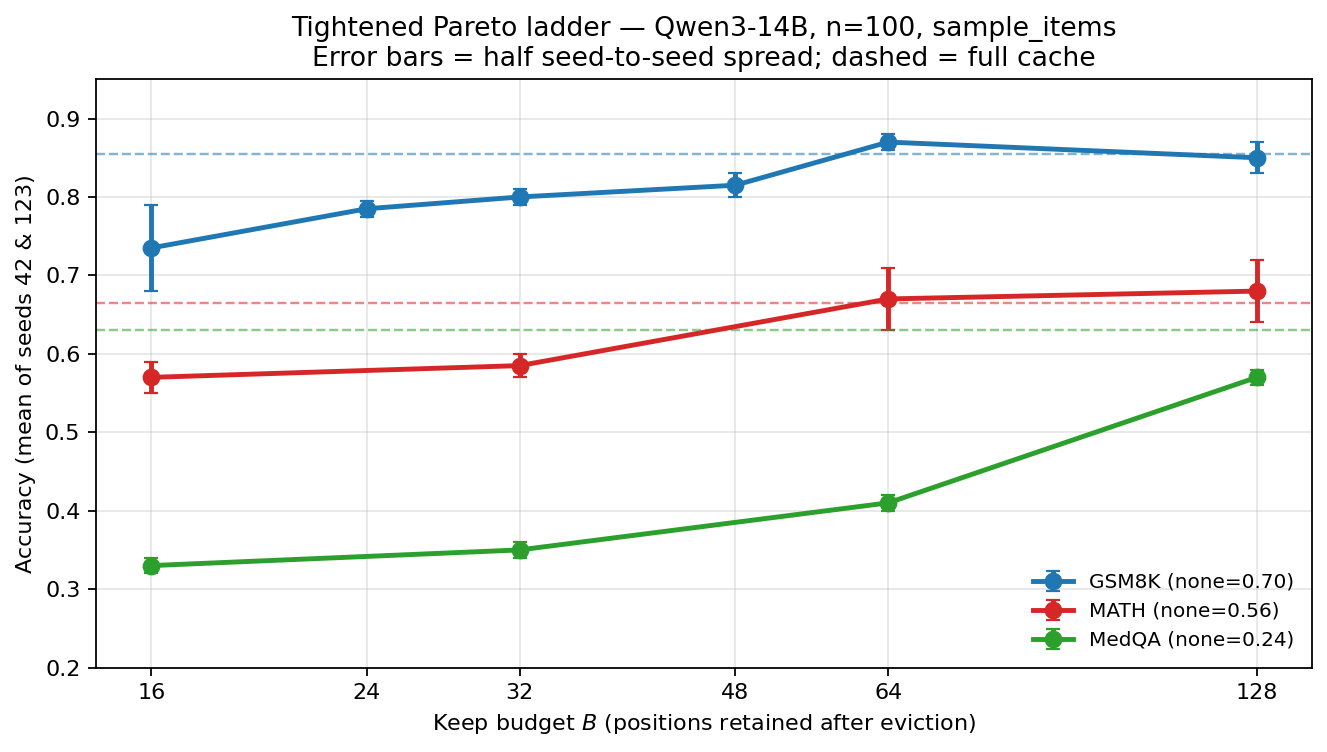
\includegraphics[width=0.92\textwidth]{pareto_acc_vs_B.png}
\end{center}
\vspace{-0.6em}
\begin{itemize}\small
  \item \textbf{GSM8K:} soft at $B{=}16$; iso by $B{\approx}64$ ($\sim\!10\times$).
  \item \textbf{MATH:} free-ish from $B{\approx}64$--$128$ ($\sim\!5$--$10\times$).
  \item \textbf{MedQA:} still $-6$\,pp at $B{=}128$ --- thickness required.
\end{itemize}
\end{frame}

\begin{frame}{Numbers (accuracy, seed-mean $n{=}100$)}
\begin{center}\small
\begin{tabular}{lrrrrrr}
\toprule
Task & full & $B{=}16$ & $B{=}32$ & $B{=}64$ & $B{=}128$ & none \\
\midrule
GSM8K & 0.855 & 0.735 & 0.800 & \textbf{0.870} & 0.850 & 0.700 \\
MATH  & 0.665 & 0.570 & 0.585 & \textbf{0.670} & \textbf{0.680} & 0.555 \\
MedQA & 0.630 & 0.330 & 0.350 & 0.410 & 0.570 & 0.240 \\
\bottomrule
\end{tabular}
\end{center}
\vspace{0.5em}
\begin{columns}[T,onlytextwidth]
\begin{column}{0.48\textwidth}
\begin{block}{\small Recommended $B$ per task}
\begin{itemize}\scriptsize
  \item GSM8K: $B{=}64$ ($\sim$10$\times$) for iso-acc
  \item MATH: $B{=}64$--$128$
  \item MedQA: $\ge 128$; avoid $16$--$64$
\end{itemize}
\end{block}
\end{column}
\begin{column}{0.50\textwidth}
\begin{alertblock}{\small Presence still matters}
\scriptsize none $\ll$ full on every task.
Compression trims redundancy; it does not delete the scaffold.
\end{alertblock}
\end{column}
\end{columns}
\end{frame}

\begin{frame}{Compression tax ($\Delta$ acc vs full)}
\begin{center}
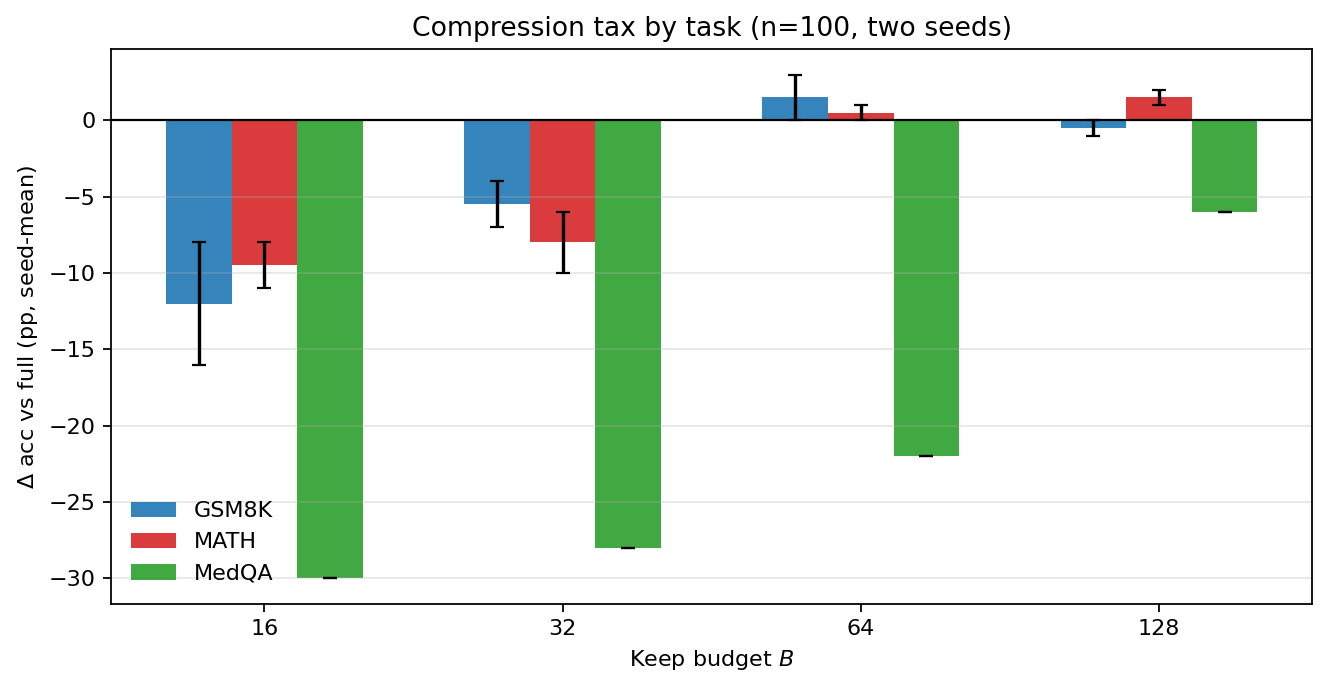
\includegraphics[width=0.88\textwidth]{pareto_delta_acc.png}
\end{center}
\end{frame}

\begin{frame}{Accuracy vs relay memory}
\begin{center}
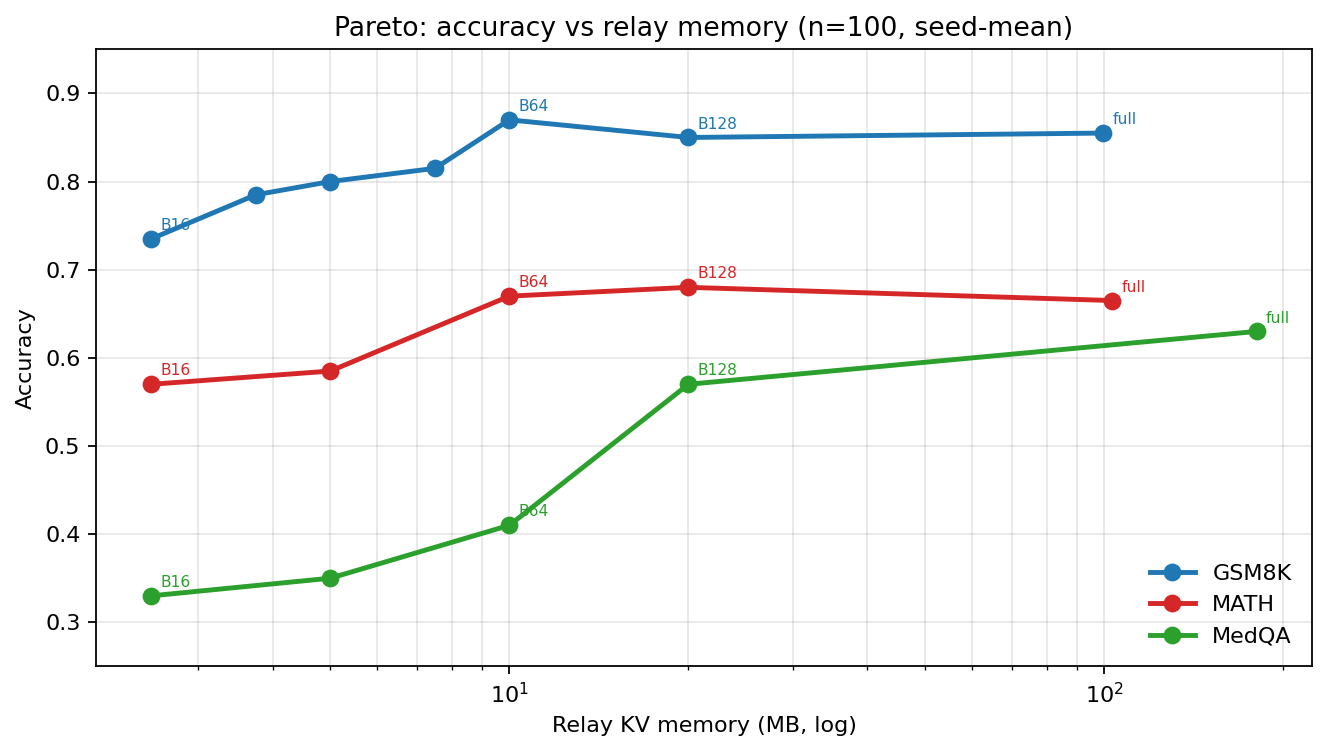
\includegraphics[width=0.90\textwidth]{pareto_acc_vs_mb.png}
\end{center}
\end{frame}

\begin{frame}{Verbosity tax (Judger tokens)}
\begin{center}
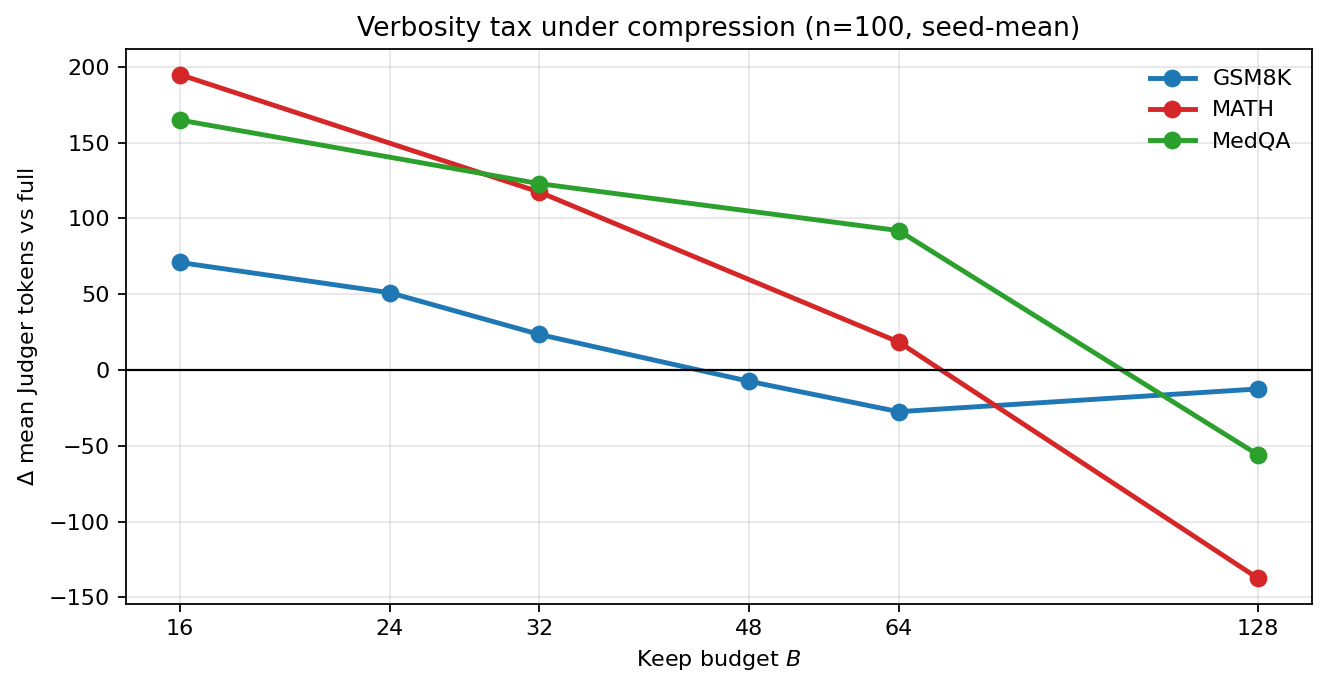
\includegraphics[width=0.88\textwidth]{pareto_token_tax.png}
\end{center}
\vspace{-0.3em}
\begin{itemize}\small
  \item Aggressive shrink lengthens Judger CoT (esp.\ MATH).
  \item Token tax fades as $B$ grows.
\end{itemize}
\end{frame}

\begin{frame}{Bottom line}
\begin{enumerate}
  \item Mechanism: relay is a scaffold, not an instance-specific channel.
  \item Systems: compress hard on easy tasks; thicker residual on hard ones.
  \item Tightened evidence ($n{=}100$, two subsets, CIs): story unchanged, sharper knees.
  \item GSM8K iso @ $B{\approx}64$ ($\sim\!10\times$); MATH @ $64$--$128$; MedQA still taxed at $128$.
\end{enumerate}
\end{frame}

\end{document}
